\documentclass[border=8pt]{standalone}
\usepackage[T1]{fontenc}\usepackage{helvet}\renewcommand{\familydefault}{\sfdefault}
\usepackage{tikz}\usetikzlibrary{arrows.meta, positioning, calc, backgrounds}
\definecolor{ink}{HTML}{1a1916}
\definecolor{inktwo}{HTML}{3a3a35}
\definecolor{inkthree}{HTML}{6a6862}
\definecolor{rule}{HTML}{b8b09a}
\definecolor{amber}{HTML}{a8730a}
\definecolor{red}{HTML}{c8261a}
\definecolor{paper}{HTML}{f0eee5}
\definecolor{slab}{HTML}{d8d4c6}
\tikzset{
  >={Stealth[length=2.2mm]},
  wire/.style={line width=0.8pt, ink},
  modwire/.style={line width=0.6pt, dashed, ink},
  tastewire/.style={line width=0.6pt, dashed, amber},
  gatewire/.style={line width=0.6pt, dotted, ink},
  block/.style={rectangle, draw=ink, line width=0.9pt, fill=slab, minimum width=3.0cm, minimum height=1.9cm, inner sep=0pt},
  perf/.style={rectangle, draw=ink, line width=0.7pt, minimum width=3.0cm, minimum height=0.7cm, inner sep=2pt, font=\footnotesize, text=ink},
  title/.style={font=\scriptsize\bfseries, text=ink, anchor=north, inner sep=2pt},
  jack/.style={circle, draw=ink, fill=paper, line width=0.5pt, minimum size=3.2pt, inner sep=0pt},
  plabel/.style={font=\tiny, text=inktwo, anchor=west, inner sep=1pt},
  olabel/.style={font=\tiny, text=inktwo, anchor=east, inner sep=1pt},
  settings/.style={font=\scriptsize, text=ink, align=left, anchor=north west, inner sep=1pt, text width=2.9cm},
}
\begin{document}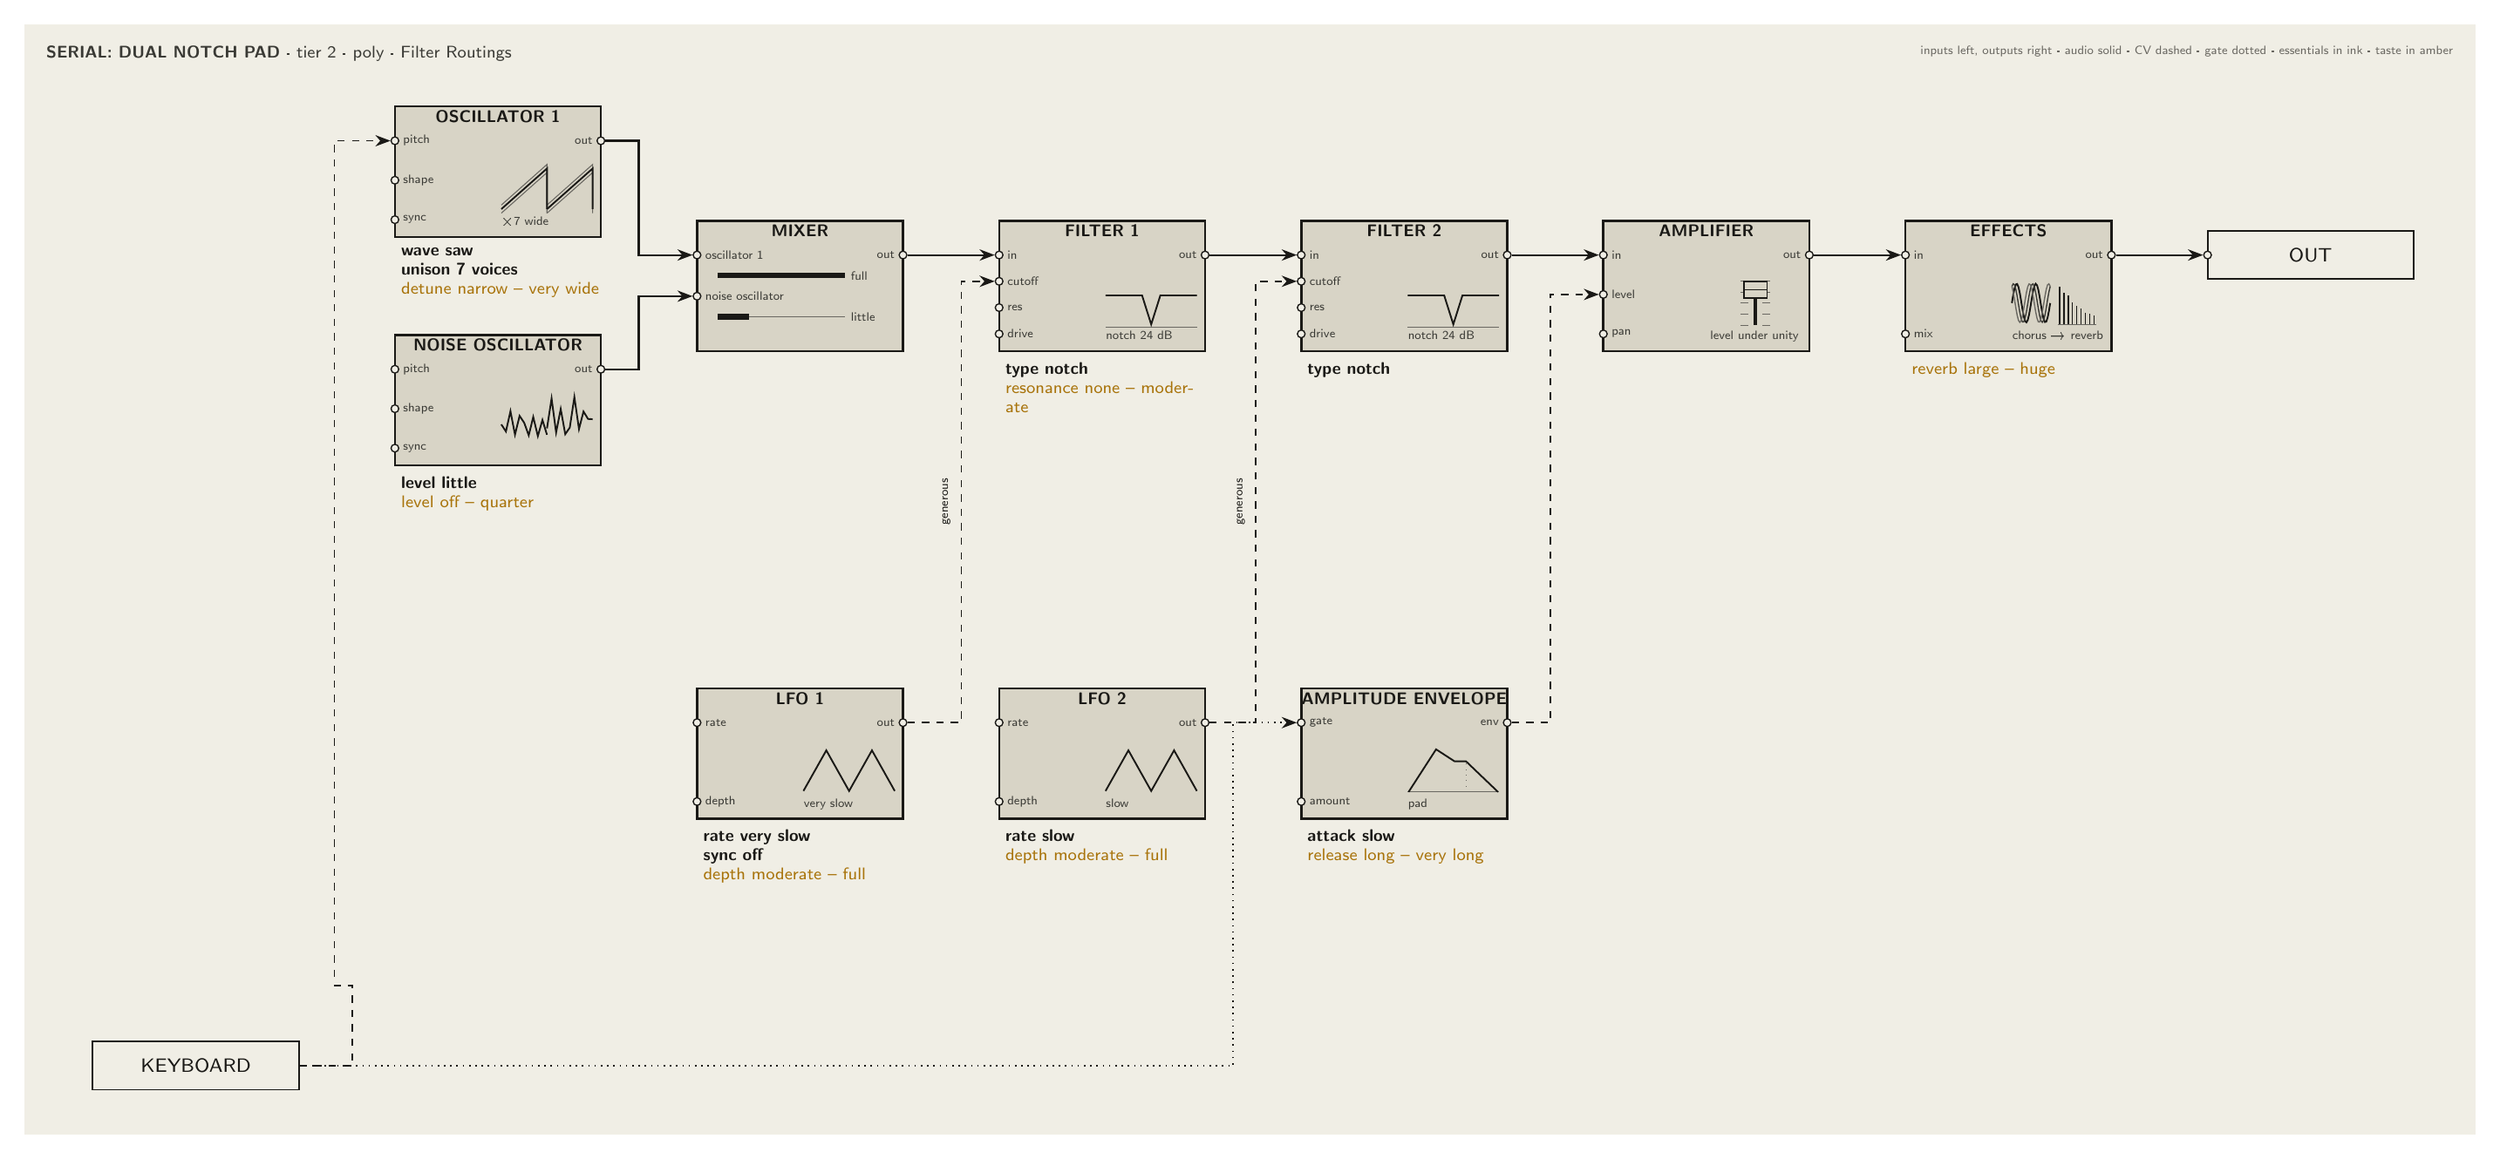
\begin{tikzpicture}
\begin{scope}[on background layer]\fill[paper] (-2.5,-12.365) rectangle (33.2,3.8150000000000004);\end{scope}
\node[block, minimum height=1.9cm] (osc1) at (4.4,1.665) {};
\node[title] at (osc1.north) {OSCILLATOR 1};
\node[jack] (osc1-pitch) at (2.9000000000000004,2.115) {};
\node[plabel] at (2.9800000000000004,2.115) {pitch};
\node[jack] (osc1-shape) at (2.9000000000000004,1.5400000000000003) {};
\node[plabel] at (2.9800000000000004,1.5400000000000003) {shape};
\node[jack] (osc1-sync) at (2.9000000000000004,0.9650000000000003) {};
\node[plabel] at (2.9800000000000004,0.9650000000000003) {sync};
\node[jack] (osc1-out) at (5.9,2.115) {};
\node[olabel] at (5.82,2.115) {out};
\begin{scope}
\draw[inkthree, line width=0.4pt] (4.450,1.178) -- (5.115,1.770) -- (5.115,1.178);
\draw[inkthree, line width=0.4pt] (5.115,1.178) -- (5.780,1.770) -- (5.780,1.178);
\draw[inkthree, line width=0.4pt] (4.450,1.060) -- (5.115,1.652) -- (5.115,1.060);
\draw[inkthree, line width=0.4pt] (5.115,1.060) -- (5.780,1.652) -- (5.780,1.060);
\draw[ink, line width=0.7pt] (4.450,1.119) -- (5.115,1.711) -- (5.115,1.119);
\draw[ink, line width=0.7pt] (5.115,1.119) -- (5.780,1.711) -- (5.780,1.119);
\node[font=\tiny, text=inktwo, anchor=north west, inner sep=0pt] at (4.450,1.015) {×7 wide};
\end{scope}
\node[settings] at (2.95,0.5950000000000001) {\textbf{wave saw} \\ \textbf{unison 7 voices} \\ \textcolor{amber}{detune narrow -- very wide}};
\node[block, minimum height=1.9cm] (noise) at (4.4,-1.665) {};
\node[title] at (noise.north) {NOISE OSCILLATOR};
\node[jack] (noise-pitch) at (2.9000000000000004,-1.215) {};
\node[plabel] at (2.9800000000000004,-1.215) {pitch};
\node[jack] (noise-shape) at (2.9000000000000004,-1.79) {};
\node[plabel] at (2.9800000000000004,-1.79) {shape};
\node[jack] (noise-sync) at (2.9000000000000004,-2.365) {};
\node[plabel] at (2.9800000000000004,-2.365) {sync};
\node[jack] (noise-out) at (5.9,-1.215) {};
\node[olabel] at (5.82,-1.215) {out};
\begin{scope}
\draw[ink, line width=0.7pt] (4.450,-2.019) -- (4.517,-2.122) -- (4.583,-1.826) -- (4.649,-2.168) -- (4.716,-1.894) -- (4.783,-1.995) -- (4.849,-2.177) -- (4.915,-1.911) -- (4.982,-2.189) -- (5.049,-1.954) -- (5.115,-2.170);
\draw[ink, line width=0.7pt] (5.115,-2.077) -- (5.182,-1.641) -- (5.248,-2.136) -- (5.315,-1.794) -- (5.381,-2.161) -- (5.447,-2.065) -- (5.514,-1.620) -- (5.581,-2.087) -- (5.647,-1.831) -- (5.713,-1.939) -- (5.780,-1.943);
\end{scope}
\node[settings] at (2.95,-2.7350000000000003) {\textbf{level little} \\ \textcolor{amber}{level off -- quarter}};
\node[block, minimum height=1.9cm] (mix) at (8.8,0.0) {};
\node[title] at (mix.north) {MIXER};
\node[jack] (mix-osc1) at (7.300000000000001,0.44999999999999996) {};
\node[plabel] at (7.380000000000001,0.44999999999999996) {oscillator 1};
\draw[inkthree, line width=0.3pt] (7.600,0.150) -- (9.450,0.150);
\draw[ink, line width=2.2pt] (7.600,0.150) -- (9.450,0.150);
\node[font=\tiny, text=inktwo, anchor=west, inner sep=1pt] at (9.500,0.150) {full};
\node[jack] (mix-noise) at (7.300000000000001,-0.15000000000000002) {};
\node[plabel] at (7.380000000000001,-0.15000000000000002) {noise oscillator};
\draw[inkthree, line width=0.3pt] (7.600,-0.450) -- (9.450,-0.450);
\draw[ink, line width=2.2pt] (7.600,-0.450) -- (8.062,-0.450);
\node[font=\tiny, text=inktwo, anchor=west, inner sep=1pt] at (9.500,-0.450) {little};
\node[jack] (mix-out) at (10.3,0.44999999999999996) {};
\node[olabel] at (10.22,0.44999999999999996) {out};
\node[block, minimum height=1.9cm] (filter1) at (13.200000000000001,0.0) {};
\node[title] at (filter1.north) {FILTER 1};
\node[jack] (filter1-in) at (11.700000000000001,0.44999999999999996) {};
\node[plabel] at (11.780000000000001,0.44999999999999996) {in};
\node[jack] (filter1-cutoff) at (11.700000000000001,0.06666666666666665) {};
\node[plabel] at (11.780000000000001,0.06666666666666665) {cutoff};
\node[jack] (filter1-res) at (11.700000000000001,-0.31666666666666665) {};
\node[plabel] at (11.780000000000001,-0.31666666666666665) {res};
\node[jack] (filter1-drive) at (11.700000000000001,-0.7) {};
\node[plabel] at (11.780000000000001,-0.7) {drive};
\node[jack] (filter1-out) at (14.700000000000001,0.44999999999999996) {};
\node[olabel] at (14.620000000000001,0.44999999999999996) {out};
\begin{scope}
\draw[inkthree, line width=0.3pt] (13.250,-0.605) -- (14.580,-0.605);
\draw[ink, line width=0.7pt] (13.250,-0.139) -- (13.782,-0.139) -- (13.915,-0.561) -- (14.048,-0.139) -- (14.580,-0.139);
\node[font=\tiny, text=inktwo, anchor=north west, inner sep=0pt] at (13.250,-0.650) {notch 24 dB};
\end{scope}
\node[settings] at (11.750000000000002,-1.0699999999999998) {\textbf{type notch} \\ \textcolor{amber}{resonance none -- moderate}};
\node[block, minimum height=1.9cm] (filter2) at (17.6,0.0) {};
\node[title] at (filter2.north) {FILTER 2};
\node[jack] (filter2-in) at (16.1,0.44999999999999996) {};
\node[plabel] at (16.18,0.44999999999999996) {in};
\node[jack] (filter2-cutoff) at (16.1,0.06666666666666665) {};
\node[plabel] at (16.18,0.06666666666666665) {cutoff};
\node[jack] (filter2-res) at (16.1,-0.31666666666666665) {};
\node[plabel] at (16.18,-0.31666666666666665) {res};
\node[jack] (filter2-drive) at (16.1,-0.7) {};
\node[plabel] at (16.18,-0.7) {drive};
\node[jack] (filter2-out) at (19.1,0.44999999999999996) {};
\node[olabel] at (19.020000000000003,0.44999999999999996) {out};
\begin{scope}
\draw[inkthree, line width=0.3pt] (17.650,-0.605) -- (18.980,-0.605);
\draw[ink, line width=0.7pt] (17.650,-0.139) -- (18.182,-0.139) -- (18.315,-0.561) -- (18.448,-0.139) -- (18.980,-0.139);
\node[font=\tiny, text=inktwo, anchor=north west, inner sep=0pt] at (17.650,-0.650) {notch 24 dB};
\end{scope}
\node[settings] at (16.150000000000002,-1.0699999999999998) {\textbf{type notch}};
\node[block, minimum height=1.9cm] (amp) at (22.0,0.0) {};
\node[title] at (amp.north) {AMPLIFIER};
\node[jack] (amp-in) at (20.5,0.44999999999999996) {};
\node[plabel] at (20.58,0.44999999999999996) {in};
\node[jack] (amp-level) at (20.5,-0.125) {};
\node[plabel] at (20.58,-0.125) {level};
\node[jack] (amp-pan) at (20.5,-0.7) {};
\node[plabel] at (20.58,-0.7) {pan};
\node[jack] (amp-out) at (23.5,0.44999999999999996) {};
\node[olabel] at (23.42,0.44999999999999996) {out};
\begin{scope}
\draw[ink, line width=1.2pt] (22.715,-0.570) -- (22.715,0.070);
\draw[inkthree, line width=0.3pt] (22.495,-0.570) -- (22.615,-0.570) (22.815,-0.570) -- (22.935,-0.570);
\draw[inkthree, line width=0.3pt] (22.495,-0.410) -- (22.615,-0.410) (22.815,-0.410) -- (22.935,-0.410);
\draw[inkthree, line width=0.3pt] (22.495,-0.250) -- (22.615,-0.250) (22.815,-0.250) -- (22.935,-0.250);
\draw[inkthree, line width=0.3pt] (22.495,-0.090) -- (22.615,-0.090) (22.815,-0.090) -- (22.935,-0.090);
\draw[inkthree, line width=0.3pt] (22.495,0.070) -- (22.615,0.070) (22.815,0.070) -- (22.935,0.070);
\fill[slab, draw=ink, line width=0.6pt] (22.545,-0.178) rectangle (22.885,0.062);
\draw[ink, line width=0.5pt] (22.545,-0.058) -- (22.885,-0.058);
\node[font=\tiny, text=inktwo, anchor=north west, inner sep=0pt] at (22.050,-0.650) {level under unity};
\end{scope}
\node[block, minimum height=1.9cm] (fx) at (26.400000000000002,0.0) {};
\node[title] at (fx.north) {EFFECTS};
\node[jack] (fx-in) at (24.900000000000002,0.44999999999999996) {};
\node[plabel] at (24.98,0.44999999999999996) {in};
\node[jack] (fx-mix) at (24.900000000000002,-0.7) {};
\node[plabel] at (24.98,-0.7) {mix};
\node[jack] (fx-out) at (27.900000000000002,0.44999999999999996) {};
\node[olabel] at (27.820000000000004,0.44999999999999996) {out};
\begin{scope}
\draw[ink, line width=0.7pt] plot[domain=0.000:0.420, samples=30, variable=\u] ({26.450+\u*1.330},{-0.620+(0.740)*(0.5+0.38*sin(360*((\u-0.000)/0.420)*2+0))});
\draw[inktwo, line width=0.5pt] plot[domain=0.000:0.420, samples=30, variable=\u] ({26.450+\u*1.330},{-0.620+(0.740)*(0.5+0.38*sin(360*((\u-0.000)/0.420)*2+60))});
\draw[inkthree, line width=0.5pt] plot[domain=0.000:0.420, samples=30, variable=\u] ({26.450+\u*1.330},{-0.620+(0.740)*(0.5+0.38*sin(360*((\u-0.000)/0.420)*2+120))});
\draw[inkthree, line width=0.3pt] (27.115,-0.561) -- (27.674,-0.561);
\draw[ink, line width=0.6pt] (27.143,-0.561) -- (27.143,-0.018);
\draw[ink, line width=0.6pt] (27.206,-0.561) -- (27.206,-0.095);
\draw[ink, line width=0.6pt] (27.269,-0.561) -- (27.269,-0.133);
\draw[ink, line width=0.6pt] (27.331,-0.561) -- (27.331,-0.246);
\draw[ink, line width=0.6pt] (27.394,-0.561) -- (27.394,-0.296);
\draw[ink, line width=0.6pt] (27.457,-0.561) -- (27.457,-0.335);
\draw[ink, line width=0.6pt] (27.520,-0.561) -- (27.520,-0.394);
\draw[ink, line width=0.6pt] (27.583,-0.561) -- (27.583,-0.408);
\draw[ink, line width=0.6pt] (27.646,-0.561) -- (27.646,-0.429);
\node[font=\tiny, text=inktwo, anchor=north west, inner sep=0pt] at (26.450,-0.650) {chorus → reverb};
\end{scope}
\node[settings] at (24.950000000000003,-1.0699999999999998) {\textcolor{amber}{reverb large -- huge}};
\node[block, minimum height=1.9cm] (lfo1) at (8.8,-6.815) {};
\node[title] at (lfo1.north) {LFO 1};
\node[jack] (lfo1-rate) at (7.300000000000001,-6.365) {};
\node[plabel] at (7.380000000000001,-6.365) {rate};
\node[jack] (lfo1-depth) at (7.300000000000001,-7.515000000000001) {};
\node[plabel] at (7.380000000000001,-7.515000000000001) {depth};
\node[jack] (lfo1-out) at (10.3,-6.365) {};
\node[olabel] at (10.22,-6.365) {out};
\begin{scope}
\draw[ink, line width=0.7pt] (8.850,-7.361) -- (9.183,-6.769) -- (9.515,-7.361) -- (9.848,-6.769) -- (10.180,-7.361);
\node[font=\tiny, text=inktwo, anchor=north west, inner sep=0pt] at (8.850,-7.465) {very slow};
\end{scope}
\node[settings] at (7.3500000000000005,-7.885000000000001) {\textbf{rate very slow} \\ \textbf{sync off} \\ \textcolor{amber}{depth moderate -- full}};
\node[block, minimum height=1.9cm] (lfo2) at (13.200000000000001,-6.815) {};
\node[title] at (lfo2.north) {LFO 2};
\node[jack] (lfo2-rate) at (11.700000000000001,-6.365) {};
\node[plabel] at (11.780000000000001,-6.365) {rate};
\node[jack] (lfo2-depth) at (11.700000000000001,-7.515000000000001) {};
\node[plabel] at (11.780000000000001,-7.515000000000001) {depth};
\node[jack] (lfo2-out) at (14.700000000000001,-6.365) {};
\node[olabel] at (14.620000000000001,-6.365) {out};
\begin{scope}
\draw[ink, line width=0.7pt] (13.250,-7.361) -- (13.583,-6.769) -- (13.915,-7.361) -- (14.248,-6.769) -- (14.580,-7.361);
\node[font=\tiny, text=inktwo, anchor=north west, inner sep=0pt] at (13.250,-7.465) {slow};
\end{scope}
\node[settings] at (11.750000000000002,-7.885000000000001) {\textbf{rate slow} \\ \textcolor{amber}{depth moderate -- full}};
\node[block, minimum height=1.9cm] (aenv) at (17.6,-6.815) {};
\node[title] at (aenv.north) {AMPLITUDE ENVELOPE};
\node[jack] (aenv-gate) at (16.1,-6.365) {};
\node[plabel] at (16.18,-6.365) {gate};
\node[jack] (aenv-amount) at (16.1,-7.515000000000001) {};
\node[plabel] at (16.18,-7.515000000000001) {amount};
\node[jack] (aenv-out) at (19.1,-6.365) {};
\node[olabel] at (19.020000000000003,-6.365) {env};
\begin{scope}
\draw[inkthree, line width=0.3pt] (17.650,-7.376) -- (18.980,-7.376);
\draw[ink, line width=0.7pt] (17.663,-7.376) -- (18.064,-6.754) -- (18.332,-6.928) -- (18.499,-6.928) -- (18.967,-7.376);
\draw[inkthree, line width=0.3pt, dotted] (18.499,-7.376) -- (18.499,-6.928);
\node[font=\tiny, text=inktwo, anchor=north west, inner sep=0pt] at (17.650,-7.465) {pad};
\end{scope}
\node[settings] at (16.150000000000002,-7.885000000000001) {\textbf{attack slow} \\ \textcolor{amber}{release long -- very long}};
\node[perf] (key) at (0.0,-11.365) {KEYBOARD};
\node[perf, fill=paper] (out) at (30.800000000000004,0.44999999999999996) {OUT}; \node[jack] (out-in) at (29.300000000000004,0.44999999999999996) {};
\draw[wire,->] (osc1-out) -- (6.45,2.115) |- (mix-osc1);
\draw[wire,->] (noise-out) -- (6.45,-1.215) |- (mix-noise);
\draw[wire,->] (mix-out) -- (filter1-in);
\draw[wire,->] (filter1-out) -- (filter2-in);
\draw[wire,->] (filter2-out) -- (amp-in);
\draw[wire,->] (amp-out) -- (fx-in);
\draw[wire,->] (fx-out) -- (out-in);
\draw[modwire,->] (lfo1-out) -- (11.15,-6.365) -- (11.15,0.06666666666666665) -- (filter1-cutoff);
\node[font=\tiny, text=ink, anchor=south, inner sep=1pt, rotate=90] at (11.030000000000001,-3.149166666666667) {generous};
\draw[modwire,->] (lfo2-out) -- (15.440000000000001,-6.365) -- (15.440000000000001,0.06666666666666665) -- (filter2-cutoff);
\node[font=\tiny, text=ink, anchor=south, inner sep=1pt, rotate=90] at (15.320000000000002,-3.149166666666667) {generous};
\draw[modwire,->] (aenv-out) -- (19.73,-6.365) -- (19.73,-0.125) -- (amp-level);
\draw[modwire,->] (key.east) -- (2.28,-11.365) -- (2.28,-10.195) -- (2.0200000000000005,-10.195) -- (2.0200000000000005,2.115) -- (osc1-pitch);
\draw[gatewire,->] (key.east) -- (15.110000000000001,-11.365) -- (15.110000000000001,-6.365) -- (aenv-gate);
\node[anchor=north west, font=\scriptsize, text=inktwo] at (-2.3,3.615) {\textbf{SERIAL: DUAL NOTCH PAD} · tier 2 · poly · Filter Routings};
\node[anchor=north east, font=\tiny, text=inkthree] at (33.0,3.615) {inputs left, outputs right · audio solid · CV dashed · gate dotted · essentials in ink · taste in amber};
\end{tikzpicture}\end{document}
